\documentclass[12pt]{article} % Default font size is 12pt, it can be changed here

\usepackage[utf8]{inputenc} % utf8 encoding
\usepackage{geometry} % Required to change the page size to A4
\geometry{a4paper} % Set the page size to be A4 as opposed to the default US Letter

\usepackage{graphicx} % Required for including pictures

\usepackage{float} % Allows putting an [H] in \begin{figure} to specify the exact location of the figure

\linespread{1.2} % Line spacing

%\setlength\parindent{0pt} % Uncomment to remove all indentation from paragraphs

\graphicspath{{pictures/}} % Specifies the directory where pictures are stored

\usepackage{listings} % To be able to have code in text
\usepackage{color} % To be able to have colors

\definecolor{codegreen}{rgb}{0,0.6,0}
\definecolor{codegray}{rgb}{0.5,0.5,0.5}
\definecolor{codepurple}{rgb}{0.58,0,0.82}
\definecolor{backcolour}{rgb}{0.95,0.95,0.92}
 
\lstdefinestyle{codestyle}{
    backgroundcolor=\color{backcolour},   
    commentstyle=\color{codegreen},
    keywordstyle=\color{magenta},
    numberstyle=\tiny\color{codegray},
    stringstyle=\color{codepurple},
    basicstyle=\footnotesize,
    breakatwhitespace=false,         
    breaklines=true,                 
    captionpos=b,                    
    keepspaces=true,                 
    numbers=left,                    
    numbersep=5pt,                  
    showspaces=false,                
    showstringspaces=false,
    showtabs=false,                  
    tabsize=2
}
 
\lstset{style=codestyle}

\begin{document}

%----------------------------------------------------------------------------------------
%   TITLE PAGE
%----------------------------------------------------------------------------------------

\begin{titlepage}

\newcommand{\HRule}{\rule{\linewidth}{0.5mm}} % Defines a new command for the horizontal lines, change thickness here

\center % Center everything on the page

\textsc{\LARGE Lund University, Faculty of Engineering}\\[1.5cm] % Name of your university/college
\textsc{\Large EDAF05}\\[0.5cm] % Major heading such as course name
\textsc{\large Algorithms, data structures, and complexity}\\[0.5cm] % Minor heading such as course title
{\large \today}\\[3cm] % Date, change the \today to a set date if you want to be precise

\HRule \\[1cm]
{ \huge \bfseries Summary of EDAF05}\\[0.4cm] % Title of your document
\HRule \\[1.5cm]

\emph{Author:} Fred \textsc{Nordell} % Your name

{\large \today}\\[3cm] % Date, change the \today to a set date if you want to be precise

%\includegraphics{Logo}\\[1cm] % Include a department/university logo - this will require the graphicx package

\vfill % Fill the rest of the page with whitespace

\end{titlepage}

%----------------------------------------------------------------------------------------
%   TABLE OF CONTENTS
%----------------------------------------------------------------------------------------

\tableofcontents % Include a table of contents

\newpage % Begins the essay on a new page instead of on the same page as the table of contents 


\section{Algorithms} % Major section

This section will describe the diffrent problems and algorithms covered in the course.

\subsection{Stable Marriage} % Sub-section
Given two sets $X = {x_{1}, x_{2}, \dots x_{n}}$ and $Y = {y_{1}, y_{2}, \dots y_{n}}$ a mathcing $M$ is a set of pairs $(x_{i}, y_{j})$ such that an $x \in X$ and an $y \in Y$ appear in most one pair. Thus it follows that a matching does not let anybody have multiple partners.

\par If the size of $M$ is $n$ it is called a \textbf{perfect matching} (All members of $X$ and $Y$ were matched). Hovever a perfect match is insufficient. All $x$ and $y$ have a preferred list, sorted in descending order, of the opposite set. The matching $M$ is considered \textbf{unstable} if it contains to pairs where they would rather switch partners. \textit{i.e.}\\
$x_{i}$ prefers $y_{j}$ and $y_{j}$ prefers $x_{i}$ \\
or \\
$y_{p}$ prefers $x_{q}$ and $x_{q}$ prefers $x_{p}$ \\
Is it always possible to find a stable matching with no unstable pairs?

\subsubsection{The Gale-Shapely algorithm}
As each person has a preferred list of partners each $x$ just needs to remember the position in the list. But as $y$ has to accept $y$ has to check if $x$ is before the current matched $x_{y}$. This may need $O(n)$ operations. A naive implementation of this algorithm may have a time complexity of $O(n^3)$ as each $x$ tries to match with each $y$ and each ask take $O(n)$ time. To reduce time complexity each $y$ should not save a prefence list, instead they should save an inverted list. Thus \texttt{[3, 2, 4, 1]} means that $x_{1}$ comes at position 3 and $x_{4}$ comes at position 1. This reduces the operation to constant time. Below is a Java implementation of the Gale-Shapely algorithm.

\begin{lstlisting}[language=Java]
public String match() {
        for(Person p: persons) {
            if(p.getId() % 2 == 0) {
                y.add(p);
            } else {
                x.addLast(p);
            }
        }
        while(x.size() > 0) {
            Person m = x.removeFirst();
            int w = (m.getPrefered()/2)-1;
            if(y.get(w).matched == null) {
                y.get(w).matched = m;
                m.matched = y.get(w);
            } else if(y.get(w).compareMatched(m)) {
                x.addLast(y.get(w).matched);
                y.get(w).matched = m;
                m.matched = y.get(w);
            } else {
                x.addLast(m);
            }
        }
        StringBuilder sb = new StringBuilder();
        for (Person w : y) {
            sb.append(w.matched.name + " -- " + w.name + "\n");
        }
        return sb.toString();
    }
\end{lstlisting}

\subsection{Greedy algorithms} % Sub-section
The definition is not trivial. Main idea is to make the best local decision at a potential cost at the global level. Herein lies the problem of finding the rule wich solves the problem optimally. There are two ways we can prove optimallity. 
\begin{enumerate}
\item If the greedy algorithm is at least as good as an optimal solution we know it is also optimal
\item Exchange argument -- transform the output of an optimal algorithm to the output of the greedy algorithm
\end{enumerate}

\subsubsection{Greedy graph algorithms}
How do we find the shortest path in a given graph? to every other node? Can we find this efficiently? Edges have weights wich can be both negative and positive (although easier with positive).

\begin{figure}[H]
\center{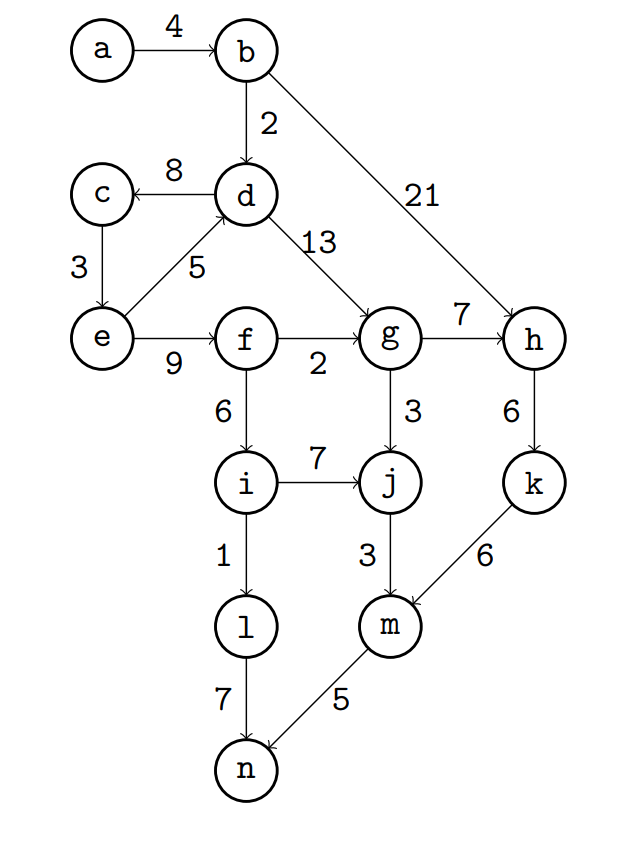
\includegraphics[width=0.5\linewidth]{graph}}
\caption{Example graph.}
\label{exgraph}
\end{figure}

\subsubsection{Dijkstra's algorithm}
Given a directed graph $G(V, E)$ a weight function $w: E -> R$ and a node $s \in V$ Dijkstra's algorithm computes the path to every other node. 

\section{Content Section} % Major section

Some more content

\subsection{Subsection 1} % Sub-section

Some more content

\subsubsection{Subsubsection 2} % Sub-sub-section

Some more content


\begin{thebibliography}{99} % Bibliography - this is intentionally simple in this template

\bibitem[Figueredo and Wolf, 2009]{Figueredo:2009dg}
Figueredo, A.~J. and Wolf, P. S.~A. (2009).
\newblock Assortative pairing and life history strategy - a cross-cultural
  study.
\newblock {\em Human Nature}, 20:317--330.
 
\end{thebibliography}

%----------------------------------------------------------------------------------------

\end{document}